% mytest

    \section{绪论}
    解析几何学是以坐标方法为基础, 运用代数方法来研究几何对象的科学. 它包含两类基本课题:(i) 从给出轨迹的集合条件,在适当的坐标系中确定它们的方程. (ii) 从给出坐标$\ x$、$y\ $ 间的方程,作出满足方程的图形. \\
    \indent 解析几何产生于十七世纪前期,当时欧洲正过渡到新的资本主义生产方式时期, 生产的发展推动了科学的进步. 当时的一些优秀科学家已经接近了解析几何的概念, 但是只有笛卡尔 ({\it Descartes}) 和费马 ({\it Fermat}) 注意到了曲线研究中的一般方法, 敏锐地发现了代数方法的必要和力量. 因此, 用代数研究几何成了他们的不二之选.\\
    \indent 笛卡尔在他的几何里解决的第一个重要课题是“帕普斯问题”, 关于这个著名的问题,古希腊人研究了它的一个特殊情况,而笛卡尔完全解决了这个问题. 但在这个问题里,笛卡尔研究的并不是点和坐标间的关系,而是线段与坐标的关系. 在他的坐标系里,对他来说,一个字母代表的永远只是一个正数. 因此,他的坐标系是不完备的. \\
    \indent 费马有比笛卡尔更为明确的坐标概念和坐标轴概念. 他早就叙述了他的解析几何思想,并解释了一般原理:“只要在某方程里出现了两个未知量, 我们就得到一个轨迹, 这两个量之一, 其末端就描绘出一条直线或曲线.”不仅如此, 他还写出了直线和二次曲线的方程,与现在的方程基本相同.\\
    \indent 当今解析几何中使用的名词是由莱布尼兹 ({\it Leibniz}) 首先提出的. 在英国的牛顿 ({\it Newton}) 的著作中第一次使用了坐标和正确地运用了纵横轴, 并对二次曲线和三次曲线进行了较为系统的研究. \\
    \indent 十八世纪中期,解析几何已经基本达到了成熟的阶段. 瑞士科学家欧拉 ({\it Euler}) 作了一些总结性研究. 1748 年他出版了《无穷小的分析入门》, 被誉为第一本解析几何课本. 此外, 欧拉还给出了平移和旋转的公式、平面代数曲线的分类、二次曲线的切线与渐近线,极坐标与参数方程等. 欧拉之后,又有许多数学家将内容继续完善,才达到了今天的样子. 十七世纪以来数学的巨大发展, 很大程度上归功于解析几何. \\
    \indent 十九世纪末,许多卓越的分析学家认为, 解析几何远远没有到达尽头, 必须研讨的一个课题是无穷维的解析几何. 于是, 这个课题急剧地发展成数学的一大分支—— 泛函分析. 而普通解析几何的更直接推广, 引出了另一个新的数学分支——代数几何. \\
    \indent 历久弥新, 解析几何依旧在数学的历史长河中闪耀.\\
    {\noindent} \rule[-10pt]{17.5cm}{0.05em}\\ \\ \\
    {\it \indent 算术符号是书写出来的图形, 而几何图形是绘画出来的公式. \hfill —— 希尔伯特\\ \\
    \indent Arithmetical symbols are written diagrams and geometrical figures are graphical formulas. \\ \rightline{—— David Hilbert}}
    
    \section{坐标系、曲线与方程}
    \subsection{平面直角坐标系}
    在初中({\it 甚至是小学}), 我们已经认识了平面直角坐标系, 但是当时我们并未给出它的定义({\it 而只是要求我们掌握它的性质和使用}), 现在我们将介绍如何定义一个平面直角坐标系. \\
    \indent 为了确定平面上点的位置, 我们通常在平面上取两条互相垂直的数轴, 它们具有公共的原点和单位长度. 通常, 我们取水平位置的一条叫做{\bf$\bm x$ 轴}或{\bf 横轴}; 取铅垂位置的一条叫做{\bf $\bm y$ 轴}或{\bf 纵轴}. $x$ 轴和$\ y$ 轴统称{\bf 坐标轴}. 我们定义$\ O$ 点为平面上的{\bf 坐标原点}, 这就构成了{\bf 平面直角坐标系}. 设平面上某点$\ P$ 向$\ x$ 轴和$\ y$ 轴分别作垂线,得垂足$\ M$ 和$\ N$. 设点$\ M$ 在$\ x$ 轴上的坐标是$\ x$, 点$\ N$ 在$\ y$ 轴上的坐标是$\ y$, 那么, $|x|$ 等于$\ P$ 点到$\ y$ 轴的距离$\ |PN|$, $|y|$ 等于$\ P$ 点到$\ x$ 轴的距离$\ |PM|$, 而$\ x\ $和$\ y\ $的符号说明了$\ P\ $点相对坐标轴的位置. 因此, $\ P\ $点的位置可以用有序实数对$\ (x,y)\ $唯一确定. 这个实数对$\ (x,y)\ $就称为$\ P\ $ 点在该直角坐标系中的{\bf 坐标}, 其中$\ x\ $称为{\bf 横坐标}, $\ y\ $称为{\bf 纵坐标}. 将上述步骤反过来,也可以由一个实数对$\ (x,y)\ $唯一确定面上的一个点. 这样, 平面内的点和所有实数对就建立起了一一对应的关系.
    \begin{figure}[h]
        \centering
        \begin{tikzpicture}
            \draw[-stealth](-2,0)--(5,0) node at (4.9,-0.3){$x$};
            \draw[-stealth](0,-2)--(0,5) node at (0.3,4.9){$y$};
            \fill (0,0) circle(1.5pt) node at (-0.3,-0.3){$O$};
            \fill (3,4) circle(1.5pt) node at (3.6,4.3){$P(x,y)$};
            \fill (0,4) circle(1.5pt) node at (-0.3,4){$N$};
            \fill (3,0) circle(1.5pt) node at (3,-0.3){$M$};
            \draw [line width=1.2pt] (0,4)--(3,4)--(3,0);
        \end{tikzpicture}
    \end{figure}\\
     \begin{figure}[h]
        \centering
        \begin{tikzpicture}
            \fill (0,0) circle(1.5pt) ;
            \fill (4.38,1.23) circle(1.5pt) ;
            \fill (0.95,-0,33) circle(1.5pt) ;
            \fill (0,-2.5) circle(1.5pt) ;
            \fill (3.8,-2.5) circle(1.5pt) ;
            \fill (2.32,2,79) circle(1.5pt) ;
            \fill (1.95,4.11) circle(1.5pt) ;
            \fill (4.55,0) circle(1.5pt) ;
            \draw (0,0) circle(4.55cm);
            \draw [line width=1.2pt] (0,4)--(3,4)--(3,0);
        \end{tikzpicture}
    \end{figure}
    {\it \indent {\bf 练习}\ \ 点的基本几何变换\\
    \indent \indent (1) 写出点$\ A(2,3)\ $关于$\ x\ $轴的对称点的坐标.\\
    \indent \indent (2) 写出点$\ A(2,3)\ $关于原点的对称点的坐标.\\
    \indent \indent (3) 写出点$\ A(2,3)\ $绕原点顺时针旋转$\ \frac{\pi}{2}\ $得到的点的坐标.\\
    \indent \indent (4) 写出点$\ A(2,3)\ $关于直线$\ x=2\ $的对称点的坐标.\\
    \indent \indent (5) 写出点$\ A(2,3)\ $关于点$\ (1,4)\ $的对称点的坐标.\\
    \indent \indent (6) 写出点$\ A(2,3)\ $绕点$\ (1,4)\ $逆时针旋转$\ \frac{\pi}{2}\ $得到的点的坐标.\\
    \indent \indent (7)* 写出点$\ (a,b)\ $关于直线$\ x=t\ $的对称点的坐标.\\
    \indent \indent (8)* 写出点$\ (a,b)\ $关于点$\ (m,n)\ $的对称点的坐标.\\}
    \subsection{曲线与方程}
    点和曲线都是我们熟知的直观几何对象, 现在我们已经通过平面直角坐标系将点“解析化”, 而曲线可以看成点按一定规律运动形成的轨迹, 因此, 曲线上的点的共同性质, 就可以反映为点$\ (x,y)\ $所满足的限制条件, 通常用二元方程$\ F(x,y)=0\ $来表示. 至此, 我们也可以完成曲线的“解析化”.\\
    \indent 我们用一个简单的例子说明. 在平面直角坐标系中, 单位圆的方程为$\ x^2+y^2=1\ $, 这就说明如果$\ P(x_{0},y_{0})\ $是单位圆上的点, 则它到原点的距离为\ 1, 由点的距离公式, 则有$\sqrt{x_{0}^2+y_{0}^2}=1$, 即$\ x_{0}^2+y_{0}^2=1$. 这说明, $\ (x_{0},y_{0})\ $是方程$\ x^2+y^2=1\ $的解. 反过来, 以这样的解为坐标的点一定在单位圆上.
    \begin{define}
    如果曲线$\ C\ $在给定的平面直角坐标系下满足下列条件: \\
    \indent (i) 曲线$\ C\ $上任意一点的坐标$\ (x,y)\ $都满足方程$\ F(x,y)=0\ $;\\
    \indent (ii) 所有满足方程$\ F(x,y)=0\ $的$\ (x,y)\ $对应的点在曲线$\ C\ $上,\\
    则称方程$\ F(x,y)=0\ $为曲线$\ C\ $的方程, 对应地, 称曲线$\ C\ $ 为方程$\ F(x,y)=0\ $ 的曲线.
    \end{define}
    \begin{figure}[h]
        \centering
        \begin{tikzpicture}
             \draw[-stealth](-1,0)--(3.5,0) node at (3.4,-0.3){$x$};
            \draw[-stealth](0,-1)--(0,3) node at (0.3,2.9){$y$};
             \fill (0,0) circle(1.5pt) node at (-0.3,-0.3){$O$};
            \draw (0.4,0.7)..controls(1,2.4)and(2.5,2.4)..(3,1.8) node at (3.9,2.2){\footnotesize $C:F(x,y)=0$};
            \fill (1,1.68) circle(1.5pt) node at (1.75,1.5){\footnotesize $P(x_{0},y_{0})$};
        \end{tikzpicture}
    \end{figure}
    {\it \indent {\bf 练习}\ \ 判断下列方程是否为所给曲线的方程\\
    \indent \indent (1) 过点$\ (0,0)\ $和$\ (2,2)\ $的线段: $x-y=0$.\\
    \indent \indent (2) 与$\ y\ $轴平行且与$\ y\ $轴距离为$\ 2\ $的直线: $|x|=2$. \\
    \indent \indent (3) 与两条坐标轴的距离的积为$\ 4\ $的点的轨迹: $xy=4$.}
    \subsection{求曲线的方程}
    求曲线的方程, 即找到这样的方程$\ F(x,y)=0\ $, 它完全表现了所给曲线的几何性质. 步骤可以用五个字简单概括: {\it 建、设、现、代、化}.\\
    \indent (1) 建: 以适当的原点和单位长度建立平面直角坐标系.\\
    \indent (2) 设: 在曲线上任取一点, 设出坐标$\ (x,y)\ $.\\
    \indent (3) 现: 将曲线上的点满足的约束条件用代数语言体现.\\
    \indent (4) 代: 将坐标$\ (x,y)\ $代入约束条件, 建立方程.\\
    \indent (5) 化: 化简方程, 并讨论特殊情况.
    \begin{liti}
    求与两定点$\ A$、$B\ $满足$\ |PA|^2-|PB|^2=k^2\ (k\in \mathbb{R})\ $的动点$\ P\ $的轨迹方程.
    \end{liti}p
    {\bf 解一} \ 以过两定点$\ A$、$B\ $的直线为$\ x\ $轴, 线段$\ AB\ $的中垂线为$\ y\ $ 轴, 建立坐标系如图.
    \begin{figure}[ht]
        \centering
        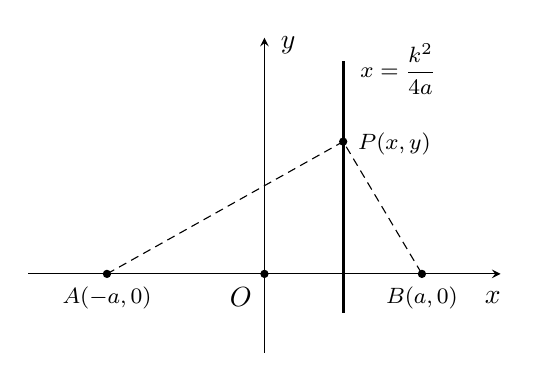
\begin{tikzpicture}
            \draw[-stealth](-3,0)--(3,0) node at (2.9,-0.3){$x$};
            \draw[-stealth](0,-1)--(0,3) node at (0.3,2.9){$y$};
            \fill (0,0) circle(1.5pt) node at (-0.3,-0.3){$O$};
            \fill (-2,0) circle(1.5pt) node at (-2,-0.3){\footnotesize $A(-a,0)$};
            \fill (2,0) circle(1.5pt) node at (2,-0.3){\footnotesize $B(a,0)$};
            \fill (1,1.68) circle(1.5pt) node at (1.65,1.65){\footnotesize $P(x,y)$};
            \draw[densely dashed] (-2,0)--(1,1.68)--(2,0);
            \draw[line width=1.2pt] (1,2.7)--(1,-0.5) node at (1.7,2.6){\footnotesize $x=\displaystyle \frac{k^2}{4a}$};
        \end{tikzpicture}
    \end{figure}\\
    设$\ A(-a,0)$,$\ B(a,0)$,$\ P(x,y)$, 则$$|PA|^2=(x+a)^2+y^2, \ |PB|^2=(x-a)^2+y^2.$$
    依题意, $|PA|^2-|PB|^2=k^2$, 即$$[(x+a)^2+y^2]-[(x-a)^2+y^2]=k^2.$$
    整理后, 得$\ 4ax=k^2$. 所以$$x=\frac{k^2}{4a}$$
    即为所求点$\ P\ $的轨迹方程, 它是一条平行于$\ y\ $轴的直线.\\
    \indent {\bf 解二} \ 以过两定点$\ A$、$B\ $的直线为$\ x\ $轴, 过点$\ A\ $且垂直于$\ x\ $轴的直线为$\ y\ $轴, 建立坐标系如图.
    \begin{figure}[h]
        \centering
        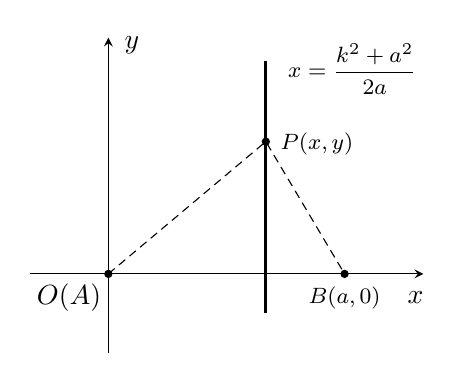
\begin{tikzpicture}
            \draw[-stealth](-1,0)--(4,0) node at (3.9,-0.3){$x$};
            \draw[-stealth](0,-1)--(0,3) node at (0.3,2.9){$y$};
            \fill (0,0) circle(1.5pt) node at (-0.5,-0.3){$O(A)$};
            \fill (3,0) circle(1.5pt) node at (3,-0.3){\footnotesize $B(a,0)$};
            \fill (2,1.68) circle(1.5pt) node at (2.65,1.65){\footnotesize $P(x,y)$};
            \draw[densely dashed] (0,0)--(2,1.68)--(3,0);
            \draw[line width=1.2pt] (2,2.7)--(2,-0.5) node at (3.1,2.6){\footnotesize $x=\displaystyle \frac{k^2+a^2}{2a}$};
        \end{tikzpicture}
    \end{figure}\\
    设$\ A(0,0)$,$\ B(a,0)$,$\ P(x,y)$, 则$$|PA|^2=x^2+y^2, \ |PB|^2=(x-a)^2+y^2.$$
    依题意, $|PA|^2-|PB|^2=k^2$, 即$$(x^2+y^2)-[(x-a)^2+y^2]=k^2.$$
    整理后, 得$\ 2ax-a^2=k^2$. 所以$$x=\frac{k^2+a^2}{2a}$$
    即为所求点$\ P\ $的轨迹方程, 它是一条平行于$\ y\ $轴的直线.\\
    \indent {\bf 注}\ \ {\it 上面的两种解法得到同一条曲线的不同方程, 这是由于坐标系选取的不同. 合适的坐标系可以使计算简化. 尝试如下图方式建立平面直角坐标系, 得到的轨迹方程如何?}
     \begin{figure}[ht]
        \centering
        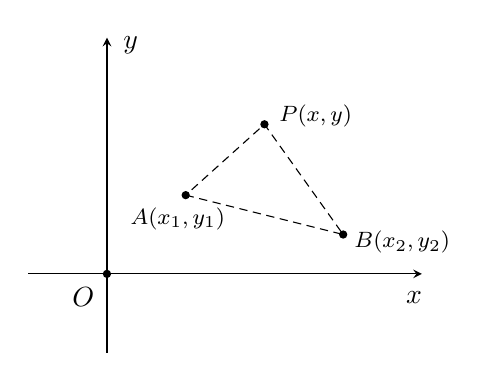
\begin{tikzpicture}
            \draw[-stealth](-1,0)--(4,0) node at (3.9,-0.3){$x$};
            \draw[-stealth](0,-1)--(0,3) node at (0.3,2.9){$y$};
            \fill (0,0) circle(1.5pt) node at (-0.3,-0.3){$O$};
            \fill (1,1) circle(1.5pt) node at (0.9,0.7){\footnotesize $A(x_1,y_1)$};
            \fill (3,0.5) circle(1.5pt) node at (3.75,0.4){\footnotesize $B(x_2,y_2)$};
            \fill (2,1.9) circle(1.5pt) node at (2.65,2){\footnotesize $P(x,y)$};
            \draw[densely dashed] (1,1)--(3,0.5)--(2,1.9)--(1,1);
        \end{tikzpicture}
    \end{figure}\\
    \begin{liti}
    给定直线$\ l\ $和它上方一点$\ F\ $, 点$\ F\ $到$\ l\ $的距离为$\ 2$. 一条在$\ l\ $上方的曲线上的点到$\ F\ $的距离减去到$\ l\ $的距离的差都是$\ 2$. 建立适当的坐标系, 求这条曲线的方程.
    \end{liti}
    {\bf 解} \ 以直线$\ l\ $为$\ x\ $轴, 过点$\ F\ $且垂直于$\ x\ $轴的直线为$\ y\ $轴, 建立坐标系如图.
    \begin{figure}[h]
        \centering
        \begin{tikzpicture}
            \draw[-stealth](-3,0)--(3,0) node at (2.9,-0.3){$x$};
            \draw[-stealth](0,-1)--(0,3) node at (0.3,2.9){$y$};
            \fill (0,0) circle(1pt) node at (-0.3,-0.3){$O$};
            \fill (2,1) circle(1pt) node at (2.4,1){$M$};
            \draw[domain=-3:3] plot(\x,0.25*\x*\x);
            \fill (0,0.7) circle(1pt) node at (-0.3,0.7){$F$};
            \fill (2,0) circle(1pt) node at(2,-0.3){$B$};
            \draw (0,0.7)--(2,1)--(2,0);
        \end{tikzpicture}
    \end{figure}\\
    设$\ M(x,y)$, 则$$|MF|=\sqrt{x^2+(y-2)^2}, \ |MB|=y.$$
    依题意, $|MF|-|MB|=2$, 即$$\sqrt{x^2+(y-2)^2}-y=2.$$
    整理后, 得$\ x^2+(y-2)^2=(y+2)^2$. 化简得$$y=\frac{1}{8}x^2.$$
    此即所求曲线的方程.\\
     \indent {\bf 注}\ \ {\it 上面的解答是典型的错误示范. 其错误在于忽略了最后一个步骤: 讨论特殊情况. 在大多数时候, 所谓特殊情况都是定义域或点的取舍问题. 在本题中, 题目要求曲线在$\ x\ $轴的上方, 即$\ y>0\ $, 但在最后的方程中, $(0,0)$为它的一个解, 却不是所求曲线上任何一点的坐标. 故不满足定义中的条件(ii). 正确的解答还应补上下面一个步骤: \\}
     \indent 因为曲线在$\ x\ $轴的上方, 所以$\ y>0\ $, 故$(0,0)$不属于所求曲线. 所以曲线的方程应是$$y=\frac{1}{8}x^2(x\not=0).$$
     {\it \indent {\bf 练习}\ \ 简单的轨迹方程求解\\
    \indent \indent (1) 已知点$\ A(-2,1)\ $和点$\ B(1,4)\ $, 求线段$\ AB\ $ 的垂直平分线的方程.\\
    \indent \indent (2) 求与距离为$\ 6\ $的两定点$\ A$、$B\ $满足$\ |PA|^2+|PB|^2=26\ $的动点$\ P\ $的轨迹方程.\\
    \indent \indent (3) 求与距离为$\ 3\ $的两定点$\ A$、$B\ $满足$\ |PA|=2|PB|\ $的动点$\ P\ $的轨迹方程. \\
    \indent \indent (4) 有一条长为$\ L\ $的木棒, 两端分别在相互垂直的两根轴上滑动. 求木棒中点的轨迹方程. }
    \subsection{本节习题}
    \begin{enumerate}
        \item 已知曲线$\ C\ $上的点的坐标都满足方程$\ F(x,y)=0$, 则下列说法正确的有
        \begin{enumerate}
            \item 不是曲线$\ C\ $上的点的坐标, 都不满足方程$\ F(x,y)=0$.
            \item 坐标满足方程$\ F(x,y)=0\ $的点都在曲线$\ C\ $ 上.
            \item 曲线$\ C\ $不一定是方程$\ F(x,y)=0\ $的曲线.
            \item $F(x,y)=0\ $不一定是曲线$\ C\ $的方程.
        \end{enumerate}
        \item 过抛物线$\ y=x^2-4\ $上任意一点$\ M\ $作$\ x\ $轴的垂线, 垂足为$\ N\ $, 求线段$\ MN\ $中点的轨迹方程.\\ \\ \\ \\ \\
        \item 已知点$\ P(x,y)\ $在单位圆$\ x^2+y^2=1\ $上, 求点$\ Q(xy,x+y)\ $的轨迹方程.\\ \\ \\ \\ \\
        \item 已知实数$\ a$、$x$、$y\ $满足$\ a^2+2a+2xy+(a+x-y){\rm i}=0$, 求点$\ (x,y)\ $的轨迹方程.\\ \\ \\ \\ \\
        \item 探究点$\ P(x,y)\ $绕原点逆时针旋转$\ \theta\ $后得到的点$\ P'(x',y')\ $的坐标.\\
        ({\it 提示: 借助和角公式或复数三角形式的运算法则.})
    \end{enumerate}
    
    \section{直线}
    \subsection{直线的确定}
    在最早接触几何时, 我们就接受了这样一条公理:\\
    \indent {\bf 直线公理}\ \ {\it 两点确定一条直线.}\\
    \indent 我们选取平面上两点$\ A(x_1,y_1)\ $和$\ B(x_2,y_2)\ $, 由直线公理可知它们可以确定一条直线. 我们在这条直线上任取一点$\ B'$, 容易发现, 对于一切选取的$\ B'$, 存在$\ \lambda\in\mathbb{R}$, 满足$\ \overrightarrow{AB}=\lambda\overrightarrow{AB'}$. 由此我们可以发现, 我们只要给定点$\ A\ $和方向向量$\ \overrightarrow{AB}$, 就可以确定直线$\ AB$.\\
    \indent “方向”体现在平面几何中, 就是一种角度关系. 当我们给定坐标系后, 就可以通过直线与坐标轴的夹角“相对地”确定直线的方向.
    \begin{figure}[h]
        \centering
        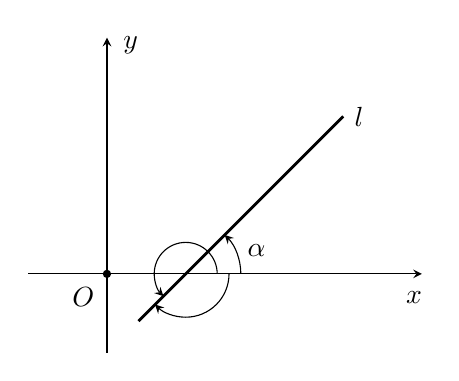
\begin{tikzpicture}
            \draw[-stealth](-1,0)--(4,0) node at (3.9,-0.3){$x$};
            \draw[-stealth](0,-1)--(0,3) node at (0.3,2.9){$y$};
            \fill (0,0) circle(1.5pt) node at (-0.3,-0.3){$O$};
            \draw[line width=1pt] (0.4,-0.6)--(3,2) node at(3.2,2){$l$};
            \draw[-stealth](1.7,0) arc(0:45:0.7) node at(1.9,0.3){$\alpha$};
            \draw[-stealth](1.4,0) arc(0:225:0.4);
            \draw[-stealth](1.55,0) arc(360:225:0.55);
        \end{tikzpicture}
    \end{figure}\\
    \indent 按这种方式, 如图, 直线$\ l\ $和$\ x\ $轴的夹角却有很多种确定方法. 对此, 我们作出如下定义:
    \begin{define}
    一条直线向上的方向和$\ x\ $轴正方向所成的最小正角, 称为这条直线的{\bf 倾斜角}, 简称{\bf 倾角}. 特别地, 当直线与$\ x\ $轴平行时, 我们规定它的倾斜角为$\ 0$.
    \end{define}
    由此我们可以知道, 对于任意一条直线, 它的倾斜角$\ \alpha\ $总满足$\ 0\leq\alpha<\pi$.
    但角度依然是一个几何化的表述. 在解析几何中, 我们更常用直线的倾斜角的正切值来刻画直线的方向.
    \begin{define}
    一条直线的倾斜角的正切值, 称为这条直线的{\bf 斜率}, 通常记为$\ k$, 即$\ k=\tan \alpha$. 特别地, 当直线与$\ x\ $轴垂直时, 斜率不存在.
    \end{define}
    我们知道, 一个方向向量可以由两点确定, 故直线的斜率可以用直线上任意两点的坐标来表示.
    \begin{figure}[h]
        \centering
        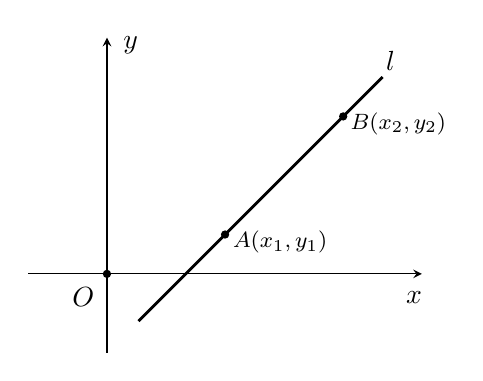
\begin{tikzpicture}
            \draw[-stealth](-1,0)--(4,0) node at (3.9,-0.3){$x$};
            \draw[-stealth](0,-1)--(0,3) node at (0.3,2.9){$y$};
            \fill (0,0) circle(1.5pt) node at (-0.3,-0.3){$O$};
            \draw[line width=1pt] (0.4,-0.6)--(3.5,2.5) node at(3.6,2.7){$l$};
            \fill (1.5,0.5) circle(1.5pt) node at(2.2,0.4){\footnotesize $A(x_1,y_1)$};
            \fill (3,2) circle(1.5pt) node at(3.7,1.9){\footnotesize$ B(x_2,y_2)$};
        \end{tikzpicture}
    \end{figure}\\
     {\it \indent {\bf 练习}\ \ 直线的斜率公式\\
    \indent \indent 已知斜率存在的直线$\ l\ $上两点$\ A(x_1,y_1),B(x_2,y_2)$, 求$\ l\ $的斜率.\\}
    \subsection{直线的方程}
    通过上一小节的探究, 我们得到了由直线两点确定的斜率公式:$$k=\frac{y_2-y_1}{x_2-x_1}.$$
    \indent 对于过点$\ A(x_0,y_0)\ $的直线$\ l$, 设其斜率为$\ k$, 则$l\ $上的点$\ P(x,y)\ $都满足$\ k=\displaystyle \frac{y-y_0}{x-x_0}.$ 整理此式, 并将点$\ A(x_0,y_0)\ $代入检验, 即得$\ l\ p$上的所有点$\ P(x,y)\ $都满足$\ y-y_0=k(x-x_0).$ 同理, 易得以方程$\ y-y_0=k(x-x_0)\ $的解为坐标的点都在直线上. 因此, 我们得到直线$\ l\ $的方程:$$y-y_0=k(x-x_0).$$
    \indent 这种形式的方程是由直线上的一点和直线斜率确定的, 顾名思义, 此即直线方程的{\bf 点斜式}.\\
    \indent 我们将点斜式方程进行变形, 得到$\ y_0-kx_0=y-kx.$ 故对$\ l\ $上的点$\ P(x,y)\ $, $y-kx\ $的值是一个常数. 我们探讨这个常数的几何意义, 令$\ x=0$, 则这个常数即为$\ x=0\ $时$\ y\ $的取值. 对应到坐标系上, 就是直线与$\ y\ $轴的交点的纵坐标. 一般地, 我们称这个纵坐标值为直线在$\ y\ $轴上的{\bf 截距}. 于是我们有理由定义$\ y_0-kx_0=y-kx=b\ $, 对点斜式方程进行变形得$\ y=kx-kx_0+y_0$, 即得:$$y=kx+b.$$
    \indent 同样, 这种形式的方程由直线斜率和直线在$\ y\ $轴上的截距确定, 故称此方程为直线方程的{\bf 斜截式}.\\
    \indent 从初中的一次函数到高中的平面解析几何, 斜截式方程贯穿始终,是较为常见的一种直线方程.\\
    \indent 现在我们回到直线的斜率公式. 我们知道, 对于确定的一条直线, 它的斜率$\ k\ $是一个定值. 故我们任取直线上的两个已知点$\ A(x_1,y_1)$、$B(x_2,y_2)$, 并任取直线上的另一点$\ P(x,y)\ $, 则我们有$$k=\frac{y-y_1}{x-x_1}=\frac{y_2-y_1}{x_2-x_1}.$$
    \indent 关于这个形式的方程的理解, 我们就可以回到最开始的直线公理了. 这样的方程是由直线上两已知点的坐标确定的, 故称此方程为直线方程的{\bf 两点式}.\\
    \indent 事实上, 对于上面所有形式的方程, 当直线的斜率存在时, 都可以通过变形化为$\ y=kx+b\ $的形式; 而如果斜率不存在, 则容易得到直线的方程可以表示为$\ x=a$. 它们的变量$\ x\ $和$\ y\ $的最高次数都不超过\ 1.由此, 我们可以得到: {\it 一切直线的方程都是关于$\ x$、$y\ $的一次方程.}\\
    \indent 那么, 一切关于$\ x$、$y\ $的一次方程是否都表示一条直线呢? 请作探究. \\
     {\it \indent {\bf 探究}\ \ 直线的一般式\\
    \indent \indent 说明任何形如$\ Ax+By+C=0\ (A,B,C\in\mathbb{R})\ $ 的方程都可以表示一条直线.\\}
\end{document}
